\subsection{Experiência 4}

Esta experiência é a junção do conhecimento das experiências anteriores para a formação de uma rede interna com duas VLAN's um computador que serve de ponte entre elas e a ligação à internet utilizando o sistema de NAT de um router comercial. O trabalho desenvolvido nesta experiência foi feito fora das aulas teórico-práticas na bancada 1.

\begin{figure}[h!]
\centering
  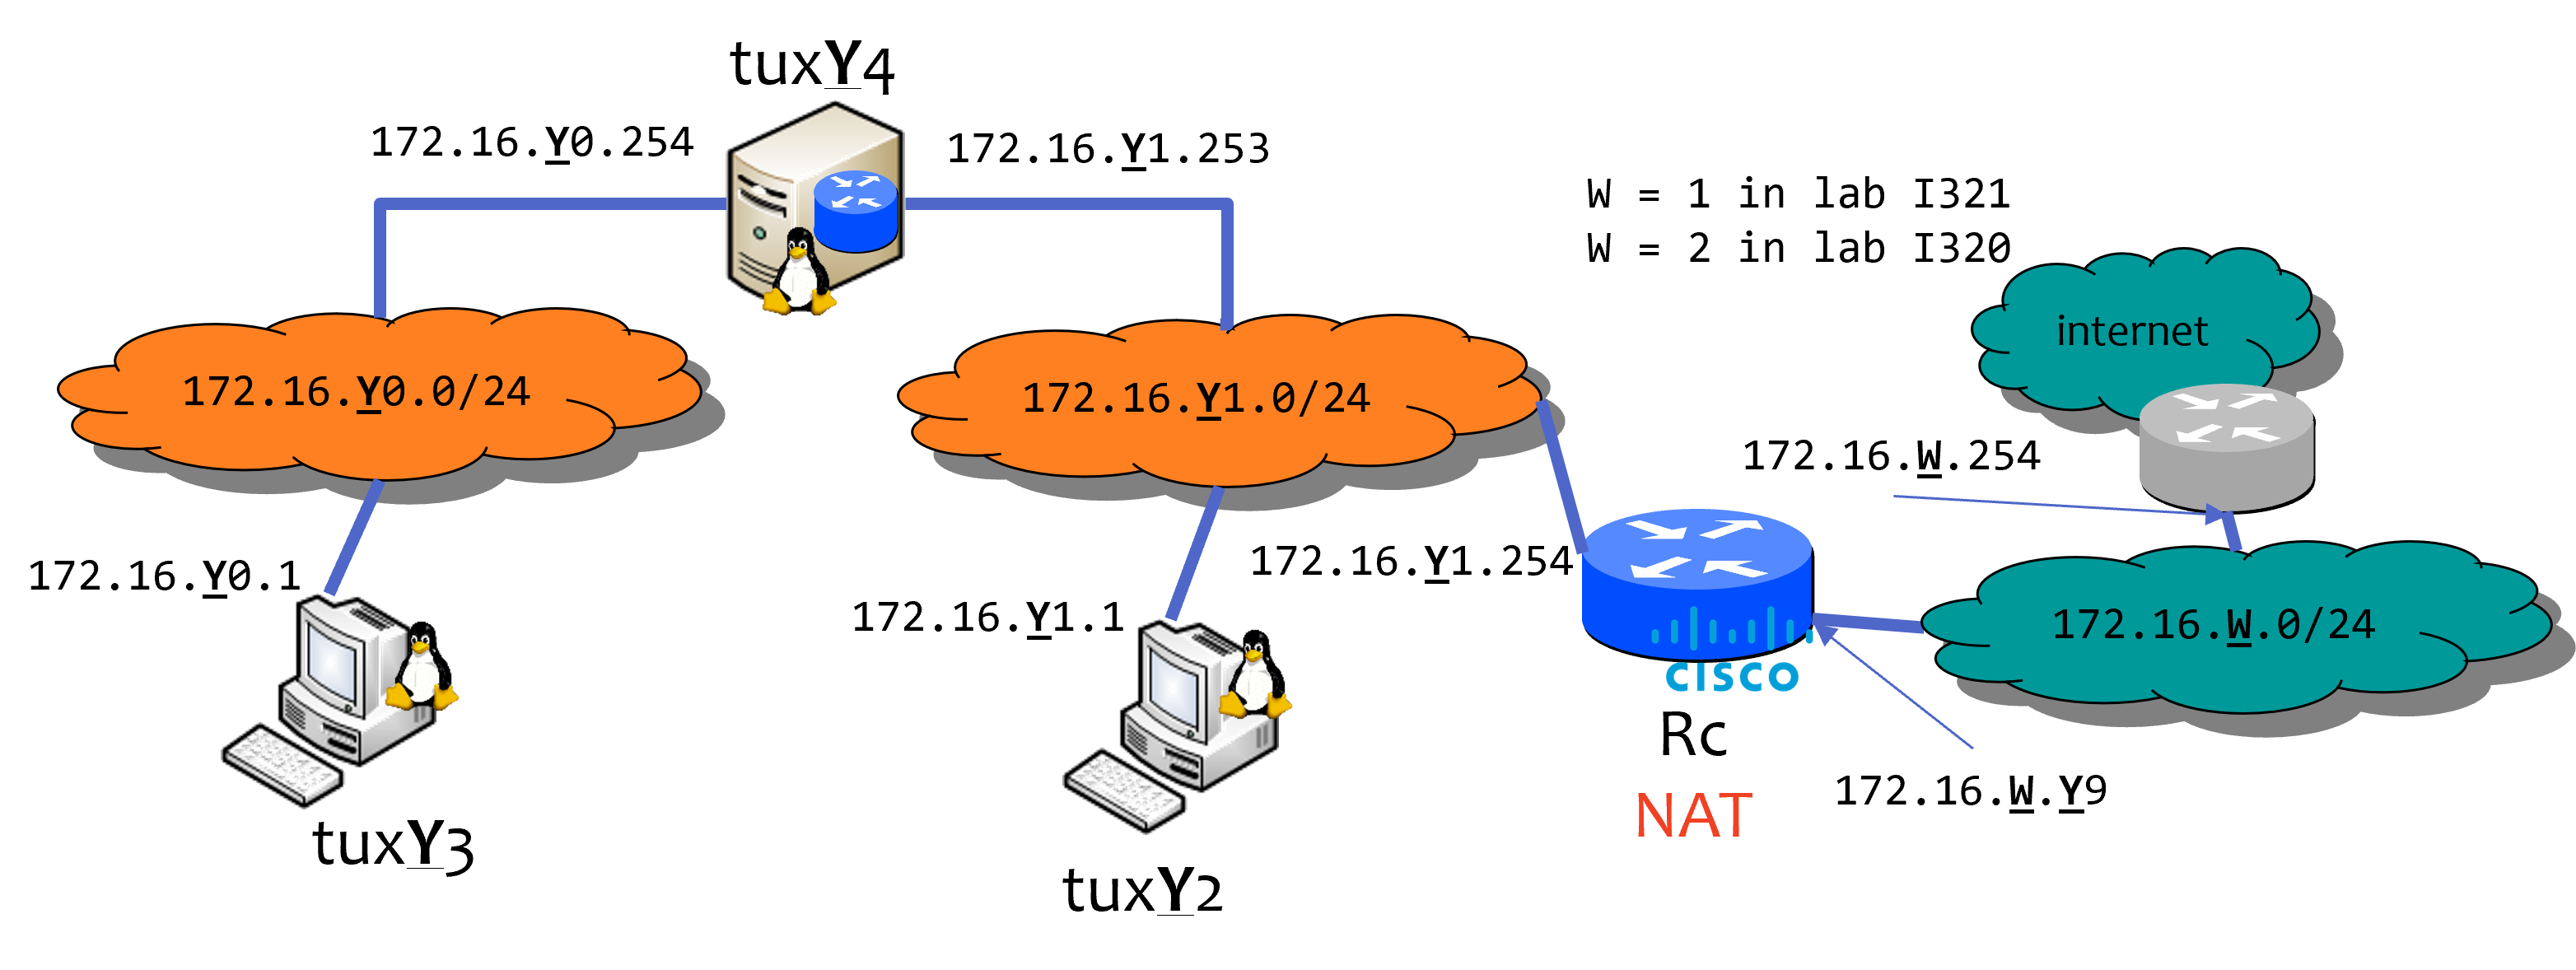
\includegraphics[width=.5\linewidth]{img/net-complete-noFTP.png}
  \caption{Estrutura da rede}
\end{figure}

\subsubsection{Questões}

\paragraph{Que rotas há nos tuxes? Qual é o seu significado?}

\paragraph{Tux52}

\begin{center}
    \begin{tabular}{ c c c }
        \textbf Destino     & \textbf Gateway       & \textbf Máscara de subrede \\ \hline
        0.0.0.0     & 172.16.11.254 & 0.0.0.0            \\
        172.16.11.0 & 0.0.0.0       & 255.255.255.0      \\
        172.16.10.0 & 172.16.11.253 & 255.255.255.0     
    \end{tabular}
\end{center}

\begin{itemize}
    \item Primeira entrada: é o endereço default, indica que todos os pacotes que não tenham match em qualquer outra rota devem ser enviados para o endereço IP 172.16.11.254 neste caso o endereço do router, que encaminhará o pacote para a internet.
    \item Segunda entrada: significa que qualquer pacote que tenha como destino a VLAN11 deve ser tratado localmente (0.0.0.0) uma vez que já atingiu a VLAN correta e não tem de ser encaminhado.
    \item Terceira entrada: significa que qualquer pacote que tenha como destino a VLAN10 deve ser enviado para o endereço 172.16.11.253 o endereço da interface do tux14 na VLAN11, uma vez que este computador é a interface entre as duas VLAN e saberá encaminhar o pacote corretamente.
\end{itemize}

\paragraph{Tux53}

\begin{center}
    \begin{tabular}{ c c c }
    \textbf Destino     & \textbf Gateway       & \textbf Máscara de subrede \\ \hline
    0.0.0.0     & 172.16.10.254 & 0.0.0.0            \\
    172.16.10.0 & 0.0.0.0       & 255.255.255.0      \\
    172.16.11.0 & 172.16.10.254 & 255.255.255.0     
    \end{tabular}
\end{center}

\begin{itemize}
    \item Primeira entrada: é o endereço default, indica que todos os pacotes que não tenham match em qualquer outra rota devem ser enviados para o endereço IP 172.16.10.254 neste caso o endereço do tux14, que encaminhará o pacote para o router.
    \item Segunda entrada: significa que qualquer pacote que tenha como destino a VLAN10 deve ser tratado localmente (0.0.0.0) uma vez que já atingiu a VLAN correta e não tem de ser encaminhado.
    \item Terceira entrada: significa que qualquer pacote que tenha como destino a VLAN11 deve ser enviado para o endereço 172.16.10.254 o endereço da interface do tux14 na VLAN10, uma vez que este computador é a interface entre as duas VLAN e saberá encaminhar o pacote corretamente.
\end{itemize}

\paragraph{Tux54}

\begin{center}
    \begin{tabular}{lll}
    \textbf Destino     & \textbf Gateway       & \textbf Máscara de subrede \\ \hline
    0.0.0.0     & 172.16.11.254 & 0.0.0.0            \\
    172.16.10.0 & 0.0.0.0       & 255.255.255.0      \\
    172.16.11.0 & 0.0.0.0       & 255.255.255.0     
    \end{tabular}
\end{center}

\begin{itemize}
    \item Primeira entrada: é o endereço default, indica que todos os pacotes que não tenham match em qualquer outra rota devem ser enviados para o endereço IP 172.16.11.254 neste caso o endereço do router, que encaminhará o pacote para a internet.
    \item Segunda entrada: significa que qualquer pacote que tenha como destino a VLAN10 deve ser tratado localmente (0.0.0.0) uma vez que já atingiu a VLAN correta e não tem de ser encaminhado.
    \item Terceira entrada: significa que qualquer pacote que tenha como destino a VLAN11 deve ser tratado localmente (0.0.0.0) uma vez que já atingiu a VLAN correta e não tem de ser encaminhado.
\end{itemize}

\paragraph{Que informação contém uma entrada da forwarding table?}

Uma entrada na forwarding table contém os seguintes dados:
\begin{itemize}
    \item Endereço de destino para uma subrede (Destination) 
    \item Máscara de subrede(Genmask)
    \item Endereço do próximo salto (Gateway)
    \item Flags associadas com ACL
    \item Métrica associada à ligação. É escolhida a entrada com a métrica menor
    \item Número de rotas que se referem aquela entrada, este valor não é usado pelo kernel Linux (Ref)
    \item Coluna com número de consultas à rota (Use)
    \item Interface de comunicação (Iface)
\end{itemize}


\paragraph{Que mensagens ARP, e endereços MAC, são observados e porquê?}

Ao fazer ping do tux13 para o tux12 capturando pacotes nas duas interfaces são observados os seguintes pacotes ARP.

Primeiro é observado um pacote que pede que o endereço MAC do IP 172.16.10.254 seja envidado para 172.16.10.1, o endereço MAC observado é 00:21:5a:61:2f:24 (Figure 24).
Isto acontece porque o tux13 está a encontrar a interface do tux14 que encaminhará o pacote enviado pelo ping para o tux12, o endereço MAC de resposta corresponde à interface eth0 de tux14.

Em seguida na mesma interface é observado o pacote ARP que pede que o endereço MAC de 172.16.10.1 seja enviado para 172.16.10.254 (Figure 26).
Isto acontece porque o tux14 necessita do endereço MAC da interface do tux13 para encaminhar a resposta do tux12 ao ping. O endereço MAC observado é 00:21:5a:61:2d:ef o endereço de eth0 do tux13.

Já em eth1 do tux14 acontece algo semelhante, o tux14 pergunta qual o endereço MAC do tux12 (Figure 23) para lhe poder encaminhar o pacote de PING e este responde com 00:21:5a:61:2e:c3, o endereço MAC de eth0 do tux12. Em seguida o tux12 pede o endereço MAC de eth1 de tux14 (Figure 25) para lhe poder enviar a resposta a PING para que esta seja encaminhada a tux13. O tux14 responde com 00:c0:df:04:20:99 o endereço MAC de eth1 do tux14.

\paragraph{Quais são os endereços IP e MAC associados aos pacotes ICMP e porquê?}

Quando o tux13 envia o pacote ICMP para o tux12 o endereço IP de origem é 172.16.10.1 o endereço de tux13 e o de destino 172.16.11.1, o endereço de tux12. O endereço MAC de origem é o endereço 00:21:5a:61:2d:ef o enderço da interface de tux13 e o de destino 00:21:5a:61:2f:24, o endereço MAC de eth0 de tux14. Isto acontece porque o endereço MAC de destino é sempre o endereço da próxima interface e não o endereço MAC correspondente ao destino final. Como os pacotes têm de passar por tux4 este é o endereço MAC de destino. O mesmo acontece com os pacotes de resposta, os endereços IP são os endereços da origem neste caso o tux12 e o de destino é o de tux13. Já o endereço MAC de origem é o endereço de eth0 de tux14 e o de destino eth0 de tux13.

Na interface eth1 de tux4 acontece algo semelhante. Os pacotes enviados por tux13 têm o seu endereço IP como endereço IP de origem e o endereço IP de tux12 como destino. Já o endereço MAC de origem é o de eth1 de tux14 e o de destino o de eth0 de tux12. O contrário acontece com os pacotes de resposta, estes possuem como endereço de IP de origem o endereço de tux12 e o de destino o de tux13. Mas o endereço MAC de origem é eth0 de tux12 e o de destino eth1 de tux14.

\paragraph{Quais são os caminhos seguidos pelos pacotes nas experiências realizadas e porquê?}

\begin{itemize}
    \item \textbf{Router CISCO para tux12 - } O caminho seguido é router $\rightarrow$ tux12 pois estes encontram-se na mesma VLAN e podem comunicar diretamente
    \item \textbf{Router CISCO para tux13 - } O caminho seguido é router $\rightarrow$ tux14 $\rightarrow$ tux13 pois o router encontra-se na VLAN11 e o tux13 na VLAN10 por isso os pacotes enviados têm de ser enviados primeiro para tux14 
    \item \textbf{Router CISCO para tux14 - } A comunicação é direta uma vez que ambos têm interfaces conectadas à mesma VLAN
    \item \textbf{Router CISCO para a 172.16.1.254 - } A comunicação pode ser feita diretamente pois o router têm uma interface ligada à VLAN onde está a máquina de endereço 172.16.1.254.
    \item \textbf{Tux13 para 172.16.1.254 - } O caminho seguido é tux13 $\rightarrow$ tux14 $\rightarrow$ router $\rightarrow$ 172.16.1.254, isto acontece porque o tux13 não tem ligação direta a 172.16.1.254 nem ao router por isso o pacote tem de ser enviado ao tux14 que o encaminhará para o router. O router por sua vez encaminha o pacote para 172.16.1.254.
    \item \textbf{Tux13 para 104.17.113.188 - } O caminho seguido é  tux13 $\rightarrow$ tux14 $\rightarrow$ router $\rightarrow$ 172.16.1.254 $\rightarrow$ ... $\rightarrow$ 104.17.113.188, a justificação para o encaminhamento até 172.16.1.254 é a mesma que na comunicação anterior, no entanto após atingir 172.16.1.254 o pacote será encaminhado para a Internet, aí fará um caminho que desconhecemos até atingir 104.17.113.188. 
\end{itemize}

 
